\documentclass[12pt, a4paper]{article}

\usepackage{import}
\usepackage{standalone}

\usepackage[top=4cm, right=2cm, bottom=2.7cm, left=2cm]{geometry}

\usepackage{wrapfig}
\usepackage{tabulary}
\usepackage{float}
\usepackage{pifont}
\usepackage{background}
\usepackage{tikz}


\pagestyle{empty}
\setlength{\parindent}{0pt}

\begin{document}
	\begin{minipage}{\textwidth}
		\section{De Zagerij \hfill\small Bron: Bebras}
			De bevers hebben een zagerij waar ze boomstammen zagen. Ze vervoeren deze boomstammen over verschillende kanalen tot aan de beverdam. Elk kanaal kan slechts een beperkt aantal boomstammen doorlaten per minuut.
			
			In het schema hieronder stelt S het startpunt voor aan de zagerij en B het eindpunt aan de beverdam. Elk kanaal wordt voorgesteld door een pijl met daarbij aangegeven hoeveel stammen er per minuut over dat kanaal kunnen passeren.
			
			\begin{figure}[H]
				\centering
				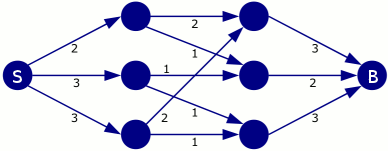
\includegraphics[width=0.8\linewidth]{image1} 
			\end{figure}

			Wat is het maximum aantal boomstammen dat elke minuut bij de beverdam kan aankomen?

			%\begin{center}
			%	Antwoord: \raisebox{-0.2cm}{\rule{5cm}{0.4pt}}
			%\end{center}

	\end{minipage} \\ \\
	
\end{document}	